\section{Building an Autonomous Vehicle Agent}
To run APEX, we need to capture the AV dynamics, the low level tracking controller, and the planning stack which generates the trajectories for the vehicle to follow. 
\subsection{Modeling}
\label{sec:model}
%We illustrate the usage of APEX by using it to verify several scenarios which cause the ego-vehicle to attempt a lane change maneuver. 
The first step towards verification is a model of the AV.
APEX uses the formalism of nonlinear hybrid systems to describe the AV and other vehicles.
The trajectory tracking controller and AV can be described using ordinary differential equations. 
The discrete nature of the behavioral control layer dictates that we much capture a system with mixed continuous-discrete dynamics. 
We provide a list of symbols used in Table \ref{table:vehiclemodel}.

\begin{table}
	\centering
	\caption{Symbols for Vehicle Model}
	\begin{tabular}{|c|c|c|}
		\hline
		\multicolumn{3}{|c|}{Symbol List} \\ \hline
		 Symbol & Units & Description \\ \hline
		$x_v$ & - & Verification State Vector \\ \hline 
		$x_{sl}$ & - & Lattice Planning State Vector \\ \hline
		$x_p$ & - & Vehicle Pose \\ \hline
		$x_g$ & - & Goal Pose \\ \hline
		$x_f$ & - & Predicted Vehicle Pose \\ \hline
		$p$ & - & Cubic Spline Parameter Vector \\ \hline
		$t_f$ & s & Prediction Horizon \\ \hline
		$m$ & kg & Vehicle Mass \\ \hline
		$l_r$ & m & Rear Wheelbase \\ \hline
		$l_f$ & m & Front Wheelbase \\ \hline
		$I_z$ & kg m$^2$ & Moment of Inertia \\ \hline
		$C_f$ & N/rad & Front Cornering Stiffness  \\ \hline
		$C_r$ & N/rad & Rear Cornering Stiffness \\ \hline
		$\beta$ & rad & Slip Angle \\ \hline
		$\Psi$ & rad & Heading Angle \\ \hline
		$v$ & m/s & Velocity \\ \hline
		$s_x$ & m & Position, x \\ \hline
		$s_y$ & m & Position, y \\ \hline
		$\delta$ & rad & Steering Angle \\ \hline
		$\epsilon_x$ & m & Tracking Error, x \\ \hline
		$\epsilon_y$ & m & Tracking Error, y \\ \hline
		$v_w$ & rad/s & Steering Angle Velocity \\ \hline 
		$a_x$ & m/s$^2$ & Longitudinal Acceleration \\ \hline
		$\kappa$ & rad/m & Curvature \\ \hline
		$s_f$ & m & Arc Length \\ \hline	
	\end{tabular}	
	\label{table:vehiclemodel}
\end{table}

\subsubsection{Ego Vehicle Model}
%To demonstrate the ability of APEX to investigate more complex vehicle models 
APEX uses a non-linear 7 degree of freedom bicycle model \cite{Rajamani2011} in order to describe the ego-vehicle. 
Higher order models can be supported in the future, and of course the parameters of the base model can be customized in order to match specific vehicles. 
See Fig. \ref{fig:bike}. 
The input to such a model is steering angle velocity and linear velocity, the output is vehicle state as a function of time. 

\begin{figure}[b]
	\centering
	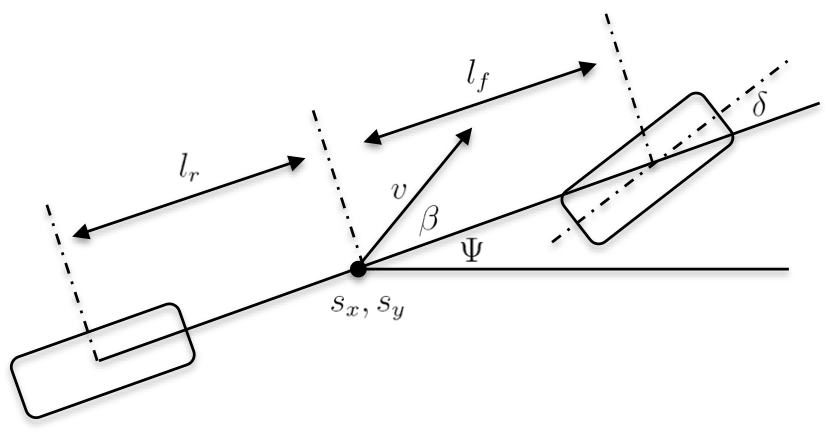
\includegraphics[scale=.6]{figures/bicycle_model.png}
	\caption{Nonlinear bicycle model describing the statespace for the APEX approach to vehicle dynamics}
	\label{fig:bike}
\end{figure}

The state vector describing the vehicle is described in equations (1)-(7). 
The variable \(\beta\) is the slip angle at the center of mass, \(\psi\) is the heading angle, \(\dot{\psi}\) is the yaw rate, \(v\) is the velocity, \(s_x\) and \(s_y\) are the x and y positions, and \(\delta\) is the angle of the front wheel. In the formulation of [6], the inputs to the system are \(a_x\), the longitudinal acceleration, and \(v_w\) the rotational speed of the steering angle. 
%The \(y\) terms represent disturbances to the system. For example \(y_{\beta}\) and \(y_{\dot{\psi}}\) represent disturbances to the slip angle at the center of mass and the yaw rate. 
\begin{equation}
	x_v = (\beta,\Psi,\dot{\Psi}, v, s_x, s_y, \delta)
\end{equation}	

 The state equations for the system as described in \cite{Althoff2014} are:
\begin{equation}
	\label{eqn:beta}
	\dot{\beta}=\left(\frac{C_rl_r-C_fl_f}{mv^2} \right)\dot{\psi}+\left(\frac{C_f}{mv} \right)\delta-\left(\frac{C_f+C_r}{mv} \right)\beta
\end{equation}
\begin{gather}
	\label{eqn:psi}
	\ddot{\psi}=\left(\frac{C_rl_r-C_fl_f}{I_z} \right)\beta-\left(\frac{C_fl_f^2-C_rl_r^2}{I_z} \right)\left(\frac{\dot{\psi}}{v} \right) \notag \\
	+\left(\frac{C_fl_f}{I_z} \right)\delta
\end{gather}
\begin{equation}
	\label{eqn:v}
	\dot{v}=a_x
\end{equation}
\begin{equation}
	\label{eqn:sx}
	\dot{s_x}=v\cos{(\beta+\psi)}
\end{equation}
\begin{equation}
	\label{eqn:sy}
	\dot{s_y}=v\sin{(\beta+\psi)}	
\end{equation}	
\begin{equation}
	\label{eqn:delta}
	\dot{\delta}=v_w
\end{equation}

%We note that in order to analyze the system we represent \(\ddot{\psi}\) as two first order differential equations. Thus we write:
%\begin{gather}
%	\dot{\psi}_{dot}=\left(\frac{C_rl_r-C_fl_f}{I_z} \right)\beta-\left(\frac{C_fl_f^2-C_rl_r^2}{I_z} \right)\left(\frac{\dot{\psi}}{v} \right) \notag \\+\left(\frac{C_fl_f}{I_z} \right)\delta\\
%	\dot{\psi}=\psi_{dot}
%\end{gather}
%Finally, one must substitute \(\psi_{dot}\) for each appearance of \(\dot{\psi}\) in the other state equations.

\subsubsection{Vehicle Parameters}
The parameters \(C_f,C_r\) and \(l_f, l_r\) describe respectively the cornering stiffness and distances from the center of gravity to the axles respectively; the subscripts $f,r$ denote whether the parameter is defined for the front or rear of the vehicle. The moment of inertia, \(I_z\) and the vehicle mass, \(m\) are experimentally determined constants \cite{Snider2009}. 
 The kinematic bicycle model considers the two front wheels and two rear wheels of the vehicle to move in unison, with steering provided by the front wheels only. Furthermore, Each abstracted wheel is located along the center of the vehicle's body. Table \ref{table:vehiclep} contains the validated vehicle parameters as given in \cite{Althoff2014}. It is possible to obtain such parameters and replace these constants in order to investigate specific vehicle characteristics. 

\begin{table}[h]
	\centering
	\caption{Parameters of Example Ego Vehicle \cite{Althoff2014}}
	\label{table:vehiclep}
	\begin{tabular}{|c|c|c|c|c|c|}
		\hline
		\multicolumn{6}{|c|}{Vehicle Parameters} \\ \hline
		\textit{$m$(kg)} & \textit{$I_z$(kg*m$^2$)} & \textit{$C_f$(N/rad)} & \textit{$C_r$(N/rad)} & \textit{$l_f$(m)} & \textit{$l_r$(m)} \\ \hline
		2273 & 4423 & 10.8e4 & 10.8e4 & 1.292 & 1.515 \\ \hline
	\end{tabular}	
\end{table}

\subsubsection{Tracking Controller}
A simple trajectory tracking controller is included with the APEX vehicle model. Trajecotry tracking controllers guide a vehicle along a geometrically defined cubic spline by apply steering and longitudinal acceleration inputs. A successful path tracking algorithm maintains vehicle stability and attempts to minimize the error between the desired trajectory and actual trajectory. The parameters computed for this controller when implemented and validated on a typical crossover SUV \cite{Althoff2014} are presented in Table \ref{table:controller}. 

\begin{table}[h]
	\centering
	\caption{Controller Parameters \cite{Althoff2014}}
	\label{table:controller}
	\begin{tabular}{|c|c|c|c|c|c|}
		\hline
		\multicolumn{6}{|c|}{Controller Parameters} \\ \hline
		$k_1$ & $k_2$ & $k_3$ & $k_4$ & $k_5$ & $k_6$ \\ \hline
		2 & 12 & 4 & 2 & 1 & 1.515 \\ \hline
	\end{tabular}	
\end{table}

%Thus, the feedback to the system are the lateral and longitudinal tracking errors. We derive the following results as in  \cite{Snider2009}:
%\begin{gather}
%	\epsilon_x=cos{(\Psi_d)}(s_{x,d}-s_x) +sin{(\Psi_d)}(s_{y,d}-s_y)
%	\\
%	\epsilon_y=-sin{(\Psi_d)}(s_{x,q}-s_x)+cos{(\Psi_d)}(s_{y,d}-s_y)
%\end{gather}



%Through the lateral tracking error, and desired trajectory we can then compute the desired rate of change of the angle of the front wheel with respect to time. This enables the computation of rate of change of the rotational speed of the steering %angle. We note that the relevant parameters are again defined using the validated model and are compiled in Table \ref{table:controller}.
%\begin{gather}
%	\delta_d=k_1 \epsilon_y+k_2(\Psi_d-\Psi)+ k_3(\dot{\Psi_d}-\dot{\Psi})
%	\\
%	v_w=k_4(\delta_d-\delta)
%	\end{gather}

%The longitudinal acceleration is simply defined by the tracking error between the actual velocity and the desired velocity.
%\begin{gather}
%	a_x=k_5\epsilon_x+k_6(v_d-v)
%\end{gather}

Using the approach in \cite{Snider2009} and \cite{Althoff2014} the control inputs for longitudinal acceleration (pressing the accelerator) and steering angle velocity (turning the steering wheel) can be computed as $v_w$ and $a_x$ respectively. 
\begin{gather}
	v_w=k_1(cos{(\Psi_d)}(s_{y,d}-s_y-w_y)-sin{(\Psi_d)}(s_{x,d}-s_x-w_x)) \notag \\ +k_2(\Psi_d-\Psi-w_{\Psi}) \notag \\ +k_3(\dot{\Psi_d}-\dot{\Psi}-w_{\psi})-k_4(\delta-w_{\delta})
	\\
	a_x=k_5(cos{(\Psi_d)}(s_{x,d}-s_x-w_x)+sin{(\Psi_d)}(s_{y,d}-s_y-w_y)) \notag \\ +k_6(v_d-v-w_v)
\end{gather}

We note that we cannot use traditional linear systems techniques or sum of squares optimizations to directly find a Lyapunov function for this system because of the obvious non-linearity and non-polynomial form of the governing ordinary differential equations. Instead we will seek to show stability and safety properties using reachability and model checking analysis.

\subsubsection{Planning}
In APEX we provide a validated planning stack which can be run on a real vehicle. The planning strategy is hierarchical and includes: mission planning, behavioral planning, and local planning. In this section we will focus on the local planner because it is the layer which connects directly to the tracking controller for the vehicle. The local planner is used to generate smooth trajectories which a non-holonomic dynamically constrained vehicle is capable of following. Our planning stack utilizes the methods outlined in 
\cite{McNaughton_2011_6927} commonly known as state-lattice planning with cubic spline trajectory generation.
%\cite{nagy2001trajectory}, , \cite{ferguson2008motion} 
\begin{figure}[t]
	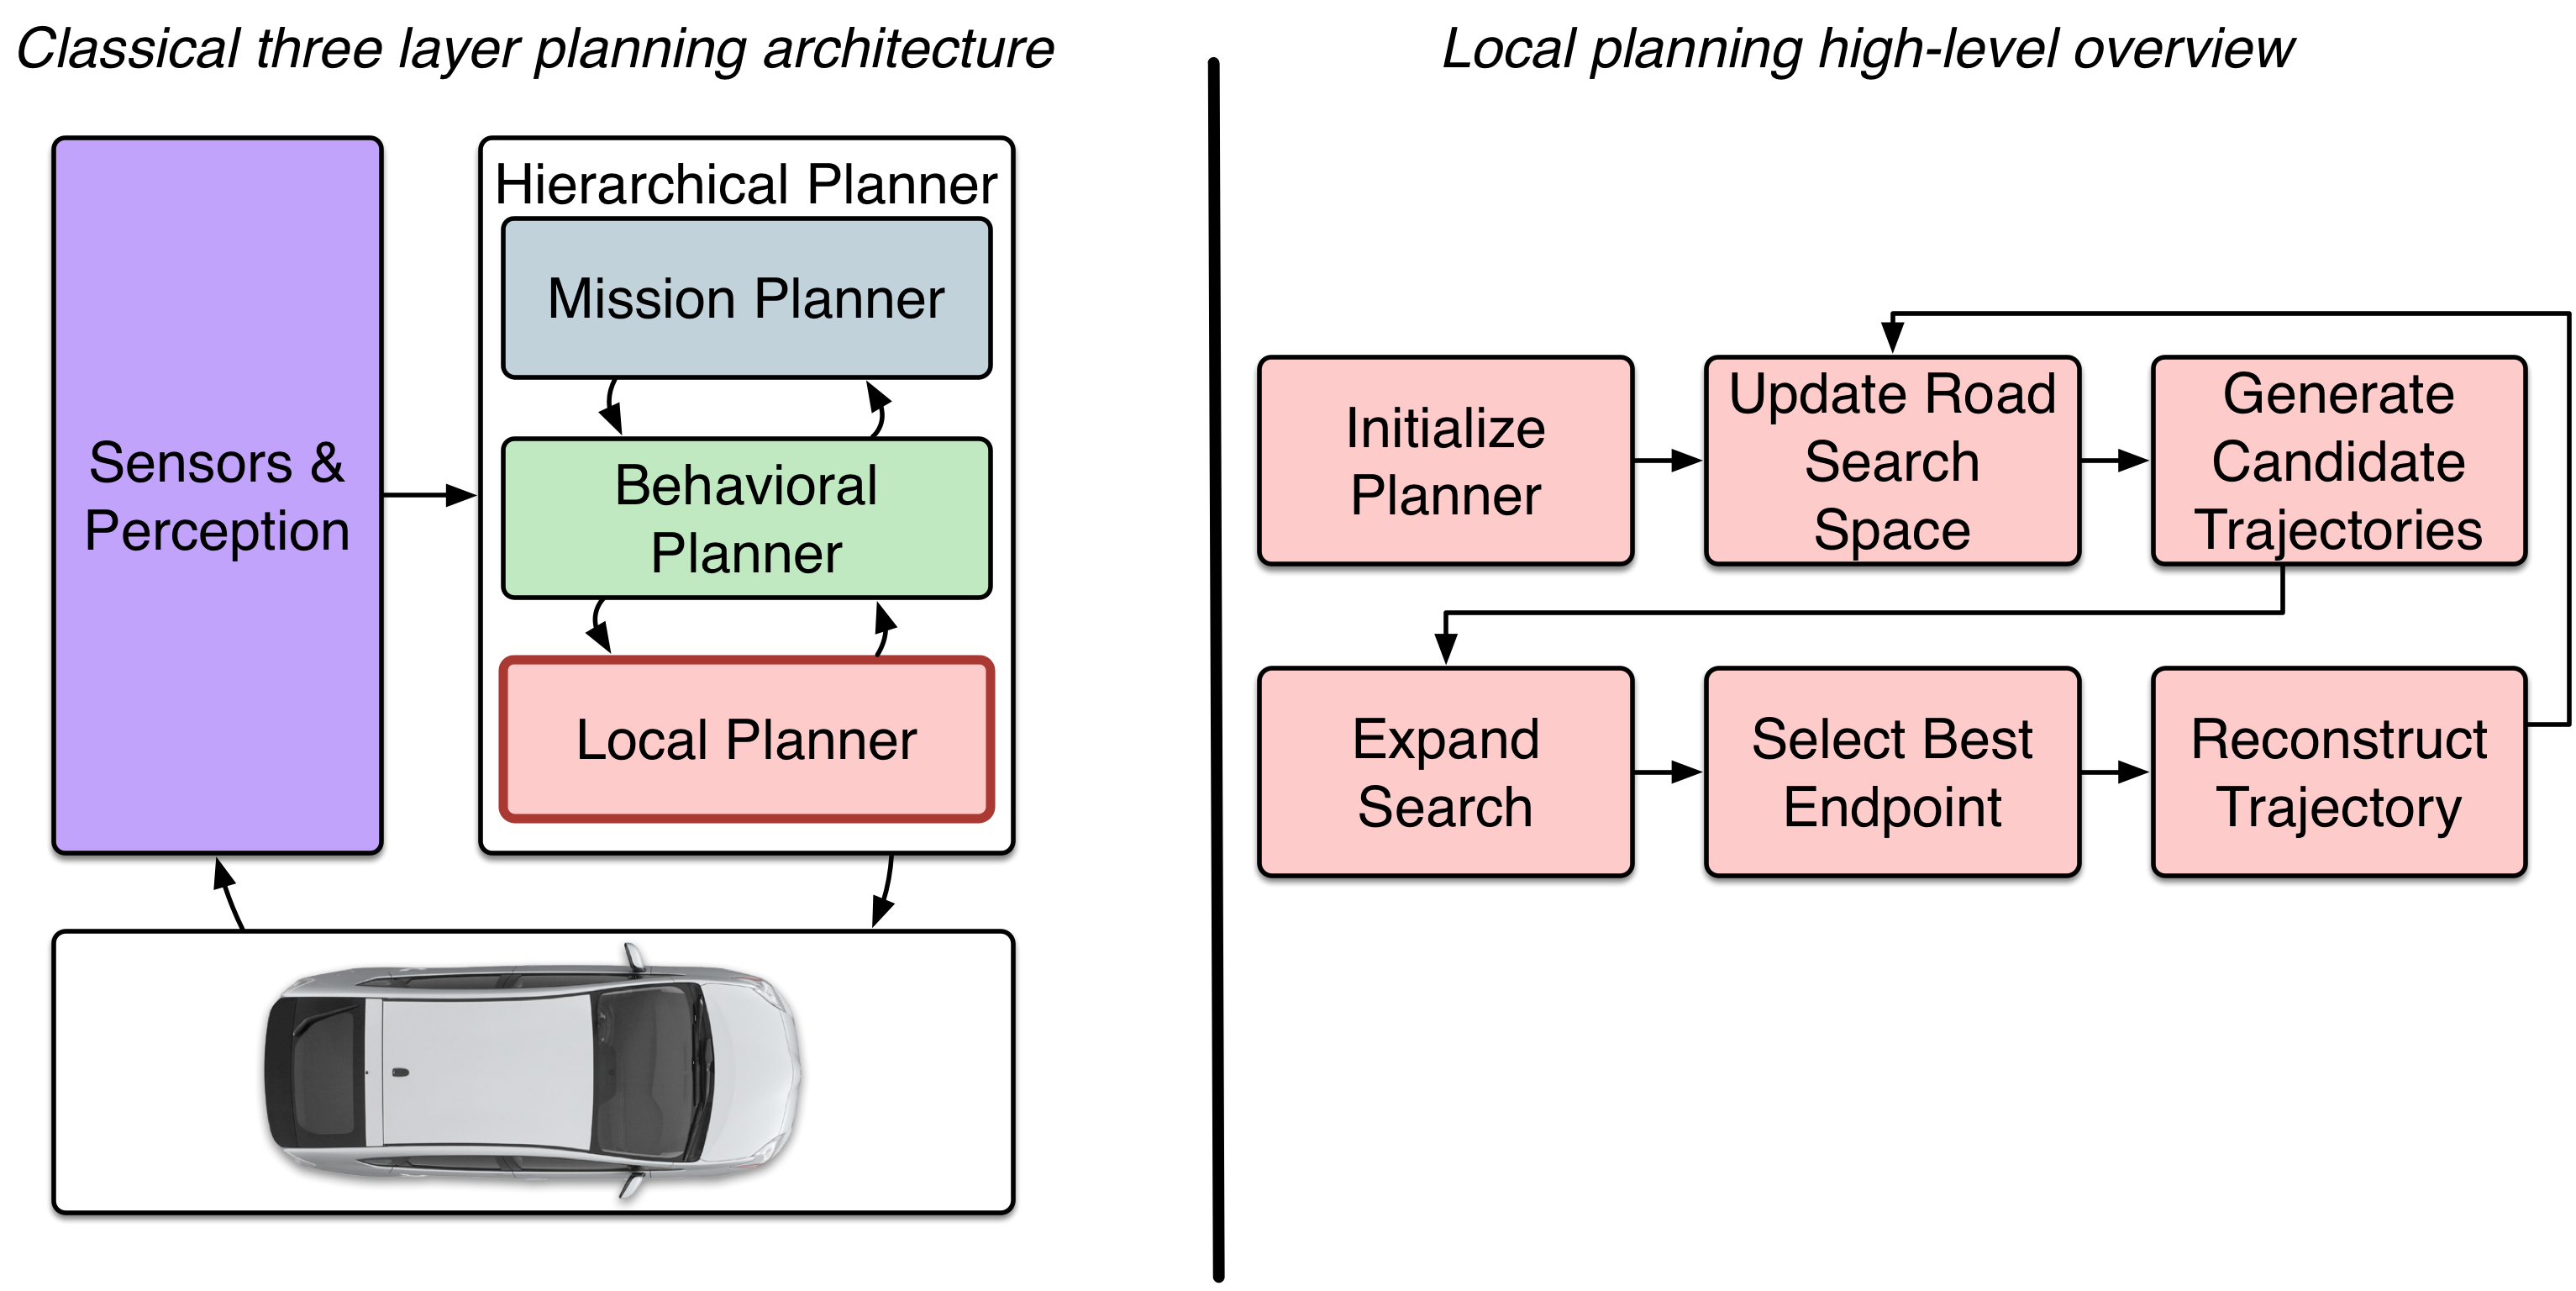
\includegraphics[width=\columnwidth]{figures/planning.png}
	\caption{Details of a local planning algorithm and used by AVs employing state lattice planning}
	\vspace{-10pt}
	\label{fig:planning}
\end{figure}

Each execution of the planner requires as an input the current state of the vehicle and a goal state as defined by the behavioral planner. We note that we will call the vehicle state $x_{sl}$ because it does not necessarily have to be the same as the model used for verification (although it can be); because the planner must run online, in real-time, lower order models are often substituted here. In this implementation we define $x_{sl}$ as:
\begin{equation}
	x_{sl}=(s_x, s_y, v, \Psi, \kappa)
\end{equation}

Where $s_x$ and $s_y$ are the x and y positions of the center of mass, $v$ is the velocity, $\Psi$ is the heading angle, and $\kappa$ is the curvature. We note that the state equations involve an additional constant, $L$ which is the wheelbase of the vehicle.
Where the state equations are described as:
\begin{equation}
	\dot{x}= v*cos(\Psi)
\end{equation}
\begin{equation}
	\dot{y} = v*sin(\Psi)
\end{equation}
\begin{equation}
	\dot{\theta}= \kappa*v
\end{equation}
\begin{equation}
	\dot{\kappa} = \frac{\dot{\Psi}}{L}
\end{equation}

The local planner's objective is then to find a feasible trajectory from the initial state defined by the tuple $x_{sl}$ to a goal pose $x_{p}$ defined as:
\begin{equation}
	x_{p} = (s_x,s_y,\Psi)
\end{equation}

In this formulation we limit trajectories to a specific class of parameterized curves known as cubic splines. A cubic spline is defined as a function of arc length:
\begin{equation}
	\kappa(s) = \kappa_0 + a \kappa_1 s + b \kappa_2 s^2 + c \kappa_3 s^3
\end{equation}

Note that there are four free parameters $(a,b,c,s_f)$ and our goal posture has four state variables. Thus, a cubic spline is a minimal polynomial that can be assured to produce a trajectory from the current position to the goal position (if it is kinematically feasible). For any particular state, goal pair there are two steps necessary to compute the parameters. First, it is necessary to produce an initial guess. There are several approaches available such as using a neural network, lookup table, or a simple heuristic. In this case we adapt a heuristic from Nagy and Kelly \cite{nagy2001trajectory} such that it is compatible with a stable parameter formulation presented by McNaughton \cite{McNaughton_2011_6927}. The stable reparameterization is defined as:
\begin{gather}
	\kappa(0)=p_0\\
	\kappa(s_f/3)=p_1\\
	\kappa(2s_f/3)=p_2\\
	\kappa(s_f)=p_3
\end{gather}

Where the parameters $(a,b,c,s_f)$ can now be expressed as:
\begin{gather}
	a(p)=p_0\\
	b(p)=-\frac{11p_0 - 18p_1+9p_2-2p_3}{2s_f}\\
	c(p)=\frac{9*(2p_0-5p_1+4p_2-p_3)}{2s_f^2}\\
	d(p)=-\frac{9(p_0-3p_1 +3p_2-p_3)}{2s_f^3}
\end{gather}
Which results in the following initialization heuristic:
\begin{gather}
	p_0=\kappa_0=\kappa_i\\ 
	p_1=\kappa_1= \frac{1}{49}(8b(s_f-s_i)-26\kappa_0-\kappa_3)\\
	p_2=\kappa_2=\frac{1}{4}(\kappa_3-2\kappa_0+5\kappa_1)\\
	p_3=\kappa_3=\kappa_f
\end{gather}

Finally, with an initial guess in hand, and a stable re-parameterization the local planner can solve a simple gradient descent problem to drive the vehicle to the goal posture. 
%We will be concerned with computing trajectories which lead from an initial state $x_i$ to a final state $x_t$ within a finite time horizon. The final state state boundary constraints which are given by the mission planner are defined by the following vector:
%\begin{equation}
%x_c=[s_x,s_y, \Psi]
%\end{equation}
%A prediction of the vehicles final state (using Euler's method) due to the control input is:
%\begin{equation}
%x_f(p,x)=x_i+\int_{t_0}^{t_f}\dot{x}(x,p)dt
%\end{equation}
%The goal of the algorithm is to drive the following equation to zero:
%\begin{equation}
%C(x,p)=x_c-x_f(p,x)
%\end{equation}
%
%We then note that $\Delta x = x_f(p,x)-x_i$ is determined by a function $f(x(p,x))$ which can be linearized such that $\Delta x = \frac{df}{dp}\Delta p$. Thus, we can iteratively update the parameters vector $p$ by the following equation:
%\begin{equation}
%	\Delta p = \frac{df}{dp}^{-1} \Delta x
%\end{equation}
%We now have a methodology for computing parameter updates, we note that the function $f(x(x,p)$ cannot be computed directly, but numerically-based algorithms exist which simplify matters. An interested reader may find the details in \cite{Howard_2009_6434}

%In Algorithm \ref{algo:estJacob} we provide the generateCorrection() function with an estimate of the Jacobian. This calculation is done numerically using a forward difference partial derivative estimate. Note that each iteration of the for loop will provide a column of the Jacobian.
%\begin{algorithm}
%	\caption{Estimate Jacobian}
%	\label{algo:estJacob}
%	\begin{algorithmic}
%		\State \textbf{estimateJacobian ($x_t, x_{t+\Delta t}, x_{goal}, u(p,x), \Delta t$)}
%		\State $ m \gets size(p)$
%		\For {$i=0; i< m; i++$}
%		\State $\frac{\delta \Delta x_{t+\Delta t}(p)}{\delta p[i]} \gets \frac{\Delta x_{t+\Delta t}(p[j]+h,p)-\Delta x_{t+\Delta t}(p)}{h}$
%		\EndFor
%		\State \Return {$\frac{\delta \Delta x_{t+\Delta t}(p)}{\delta p}$}
%	\end{algorithmic}
%\end{algorithm}	
%
%\begin{algorithm}
%		\caption{Convergence Criteria for Trajectory Generation}
%		\label{algo:checkConvergence}
%		\begin{algorithmic}
%			\State \textbf{generateCorrection ($x_t, x_{t+\Delta t}, x_{goal}, u(p,x), \Delta t$)}
%			\While {checkConvergence() = FALSE}
%			\State $\Delta x_{t+\Delta t} \gets x_{goal}-\left[x_t+\int_{t}^{t+\Delta t}f(x(t),u(p,x,t),t)dt\right]$
%			\State $\frac{\delta \Delta x_{t+\Delta t}(p)}{\delta p} \gets$ estimateJacobian()
%			\State $\Delta p = \gets -\frac{\delta \Delta x_{t+\Delta t}(p)}{\delta p}^{-1} \Delta x_{t+\Delta t}$
%			\State $ p \gets p + \Delta p$
%			\EndWhile
%			\State \Return {$p$}
%		\end{algorithmic}
%		
%\end{algorithm}
%In Algorithm \ref{algo:checkConvergence} we compute the difference between our forward motion models prediction of the future state of the vehicle and desired goal. While this difference does not satisfy the convergence criteria we update the control input parameters. Informally this is achieved by solving a system of equations which approximates how the state error will change with respect to small changes in the control parameters.

	
Thus, we can now compute a set of parameterized trajectories which may each be evaluated to test for safety and optimality. A description of these aspects of the planner may be found in \cite{McNaughton_2011_6927} and such a cost function can obviously be modified based on the goals of the design team. 
We note that our algorithm implementation is parallelized using OpenMP such that multiple trajectories (with goals regularly sampled around the initial goal) may be evaluated simultaneously. Furthermore, with small changes we can also support quintic splines which expand the variety of possible maneuvers and are more suitable for high speed driving. Figure \ref{fig:traj_gen} shows an example of a trajectory generation instance.
\begin{figure}[t]
	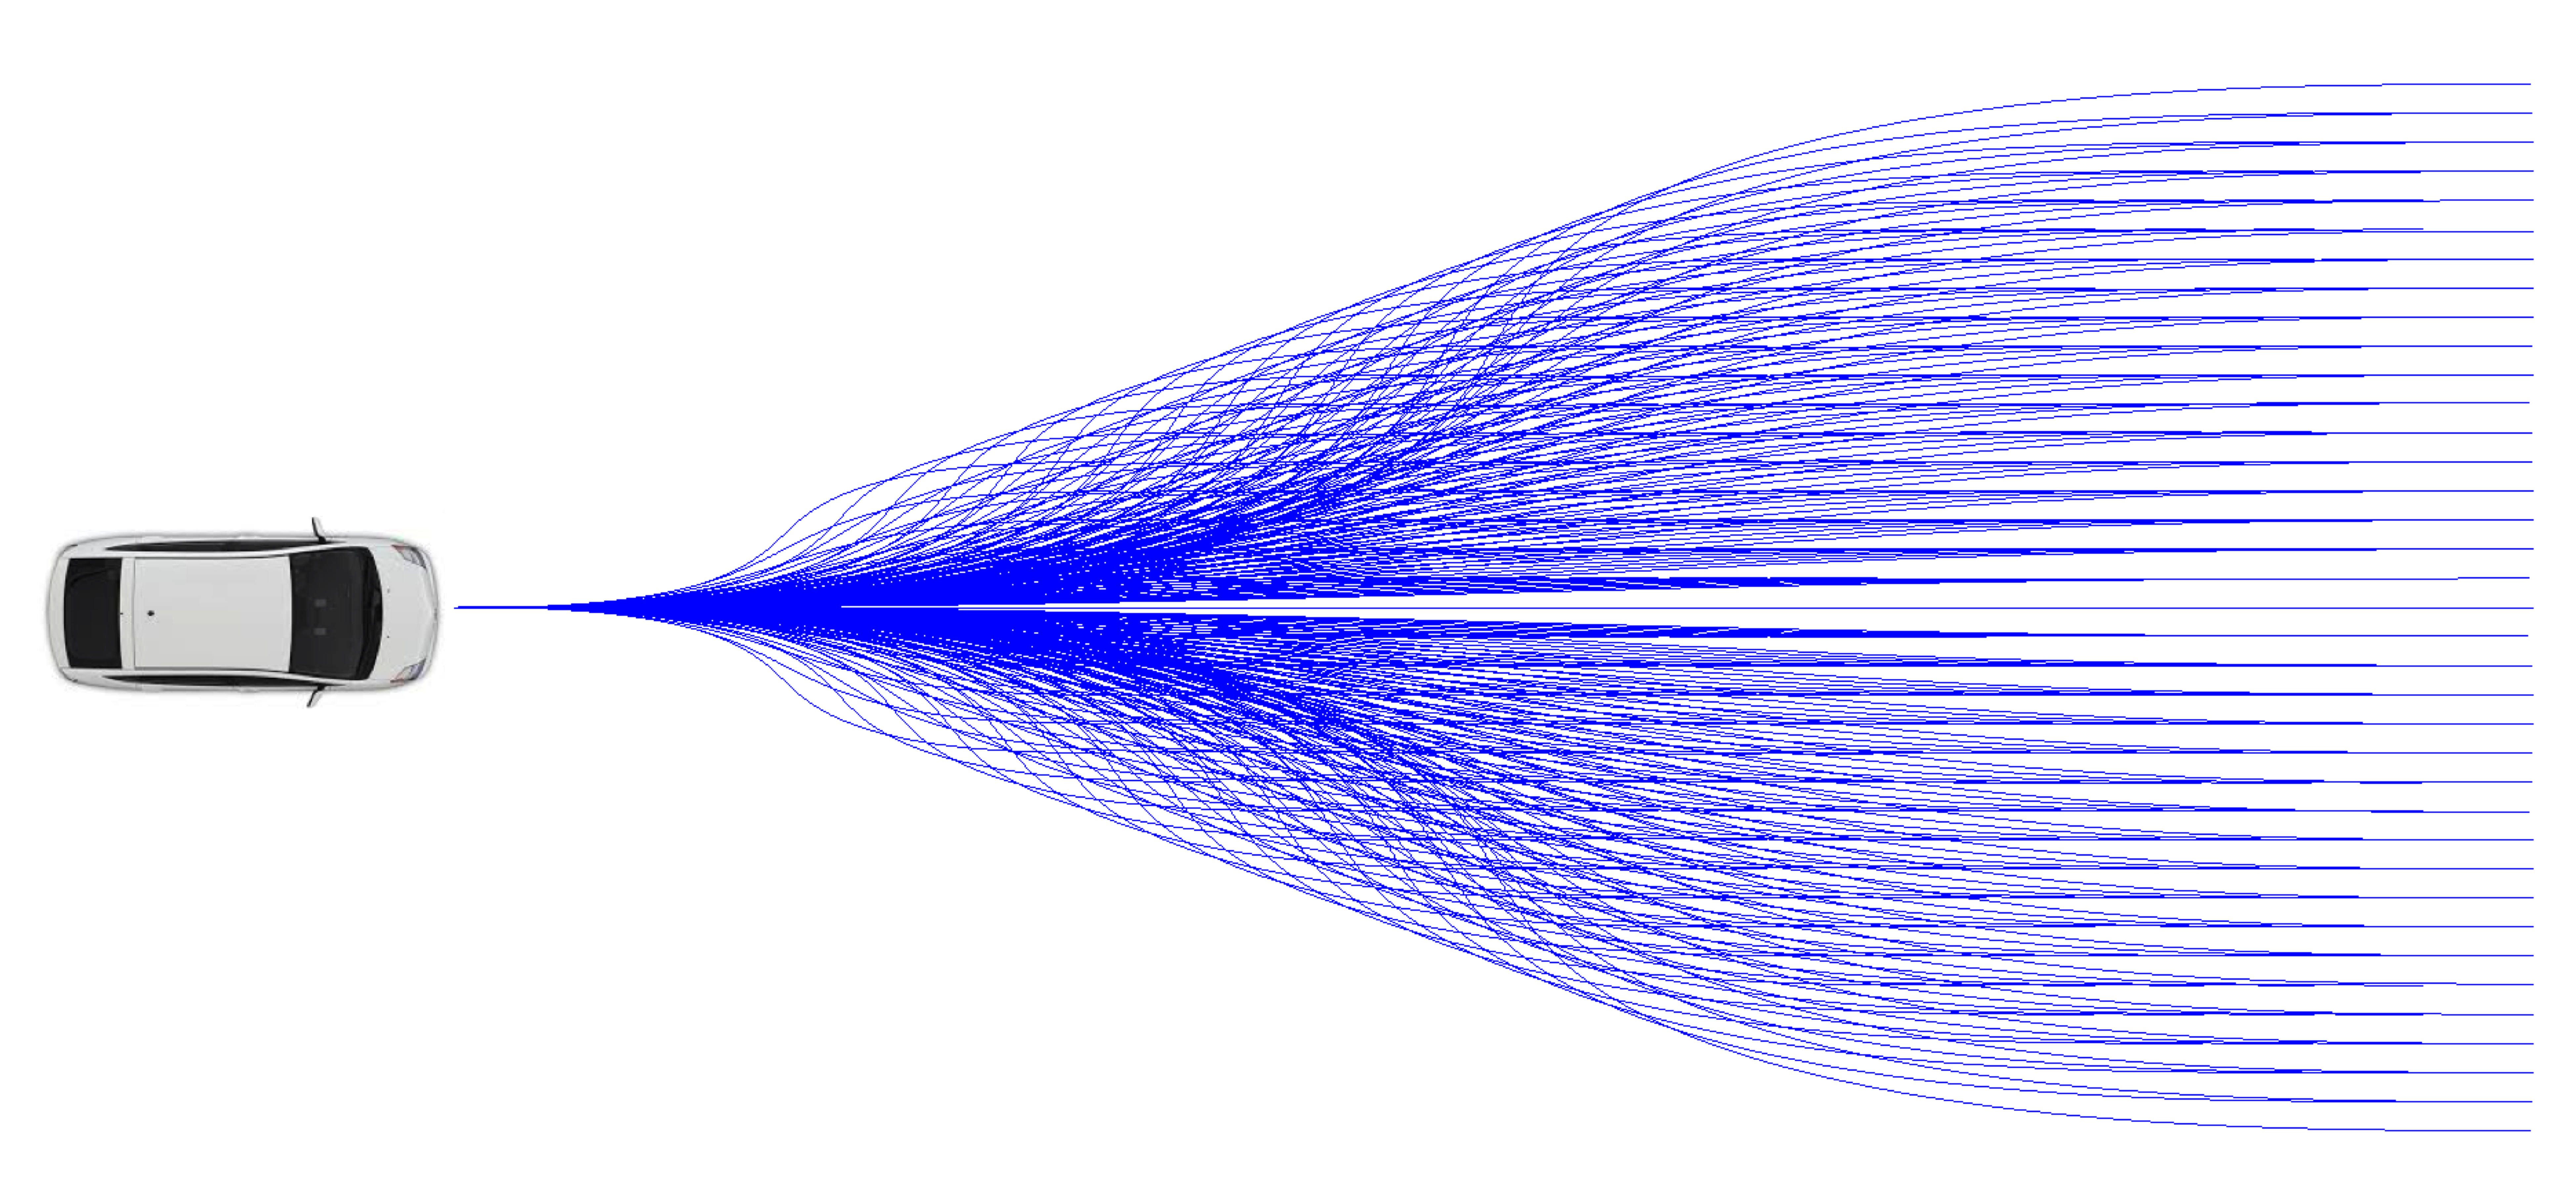
\includegraphics[width=\columnwidth]{figures/traj_gen.png}
	\vspace{-20pt}
	\caption{Output of an execution (10 Hz) of the trajectory generator, a single trajectory will be chosen from this set.}
	\label{fig:traj_gen}
\end{figure}
